\subsection{Human cost}
The human cost we analyze represents the amount of work in days and the remuneration of everyone involved in the realization of, based on our project planning, the two parts (the initial part with the management plan, and the executive plan with the installation and monitoring of one assembly line, and the formation of the employees to the handling of the machines).
The costs are based on the total number of days of work,the persons involved, and the average price cost of the employees which you can see in this table.

\begin{figure}[h]

\centering
\includegraphics[scale=1]{Img/humanCost.png}
\caption{Average employee cost}

\end{figure}

To calculate the cost we used the working rules in France and China :
\begin{itemize}
	\item[--] In France : 35 hours of work per week and 272 days of work per year.
	\item[--] In China :  40 hours of work per week and an average of 345 days of work per year. \\
\end{itemize}

The next table will present the different type of actors (employees) of this project and how much they are paid per hour according to the average employee cost of the previous table and the working rules for each country.

\begin{figure}[h]

\centering
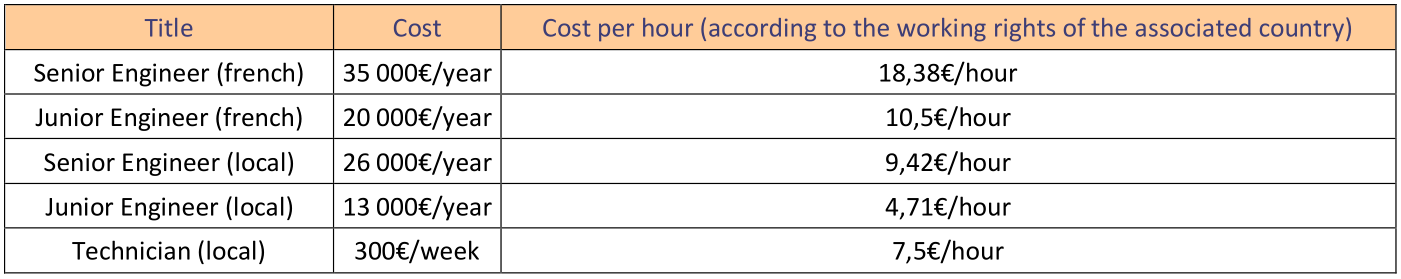
\includegraphics[scale=0.6]{Img/HumanCostPerHours.png}
\caption{Average employee costs per hour}

\end{figure}

With this data, we now analyze the number and type of the actors of each part and calculate the total cost.

\subsubsection{Initial part}
	The initial part took place during 4 days and involved a team of five french engineers, one leader senior engineer and four junior engineers.
	The cost is calculated according to the french working rule of 35 hours of work a week, so 7 hours a day.

	\begin{figure}[h]

	\centering
	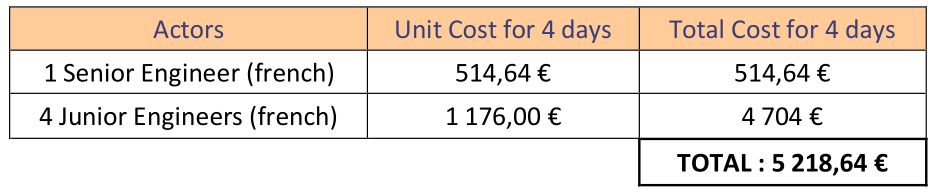
\includegraphics[scale=0.6]{Img/firstPartHumanCost.png}
	\caption{Initial part cost}

	\end{figure}

\subsubsection{Executive part}
	According to the gantt diagram, the executive part is 102 days long, minus 80 days of equipment shipping (twice 40 days), it represents 22 days of work.
	During these 22 days, 7 chinese engineers and 10 chinese technicians/regular employees (counted as technicians), as you can see here, we estimated these numbers while partitionning the executive part (installation and monitoring/control) in different tasks. \\

	\begin{figure}[h]

	\centering
	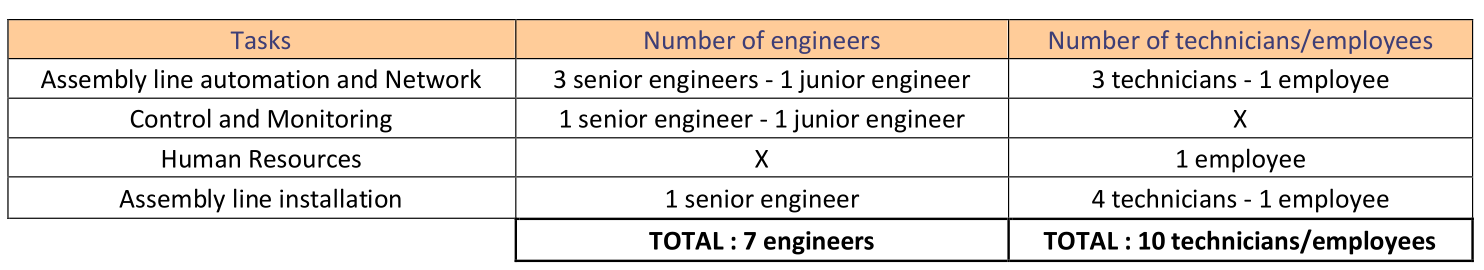
\includegraphics[scale=0.6]{Img/secondPartNbrHuman.png}
	\caption{Number of employees for the executive part}

	\end{figure}

	The cost is calculated according to the chinese working rule of an average of 40 hours of work a week, so 8 hours a day.

	\begin{figure}[h]

	\centering
	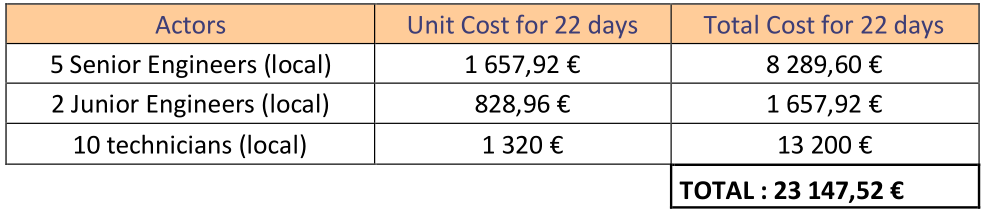
\includegraphics[scale=0.6]{Img/secondPartHumanCost.png}
	\caption{Executive part cost}

	\end{figure}

\subsubsection{Formation}
	The 17 employees involved in the executive part need to be tought how an assembly line works, how to handle the machines, how they work and also their security rules. 

	We estimated the cost of such a formation of 3000 euros per person (a total of 51 000 euros for the 17 employees) and 5 days, also counted as 5 days of works for them.

	\begin{figure}[h]

	\centering
	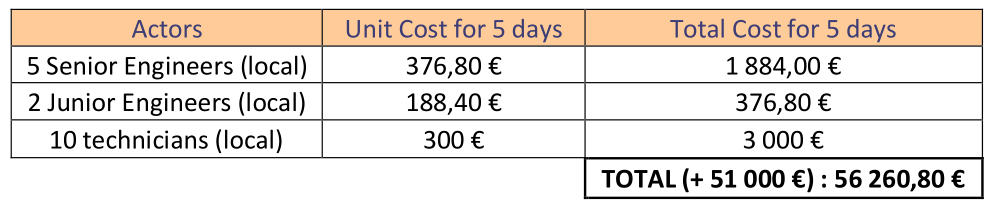
\includegraphics[scale=0.6]{Img/formationCost.png}
	\caption{Formation cost}

	\end{figure}

With these three parts, we reach a total human cost of \textbf{84 626.96 euros.} \\

\subsection{Material cost}
This cost is about every material directly used in one assembly line and its cost.
Our assembly line will include : \\
\begin{itemize}
	\item[--] Handle molds, to make the brush handle (an average of 2 per injection machine).
	\item[--] An injection machine, to mold the shape of the toothbrushes.
	\item[--] A tufting machin to tuft on brush holders.
	\item[--] A trimming and end rounding machine to cut and shape the bristles to the manufacturers specification, and to round them to be softer and more comfortable to the teeth.
	\item[--] A fully automated packaging machine to pack the toothbrushes.
	\item[--] And of course conveyers belt which will link these machines together. We estimated an average of 4 meters between machines, so we would need around 16 meters of it. \\
\end{itemize}

All of it would be around 30 square meters. \\
We have access to two types of injection machines, a 50T and a 80T, which means it is a 50/80 ton servo-motor operated machine, the maximum clamping force with these machines is either 50 or 80 tons. Servo-motors are used for energy saving, so these machines give the highest energy saving in hydraulic machines. In this estimation we chose the 80T injection machine for a better energy saving.

To calculate the total cost, we used this table of average prices. \clearpage

\begin{figure}[h]

	\centering
	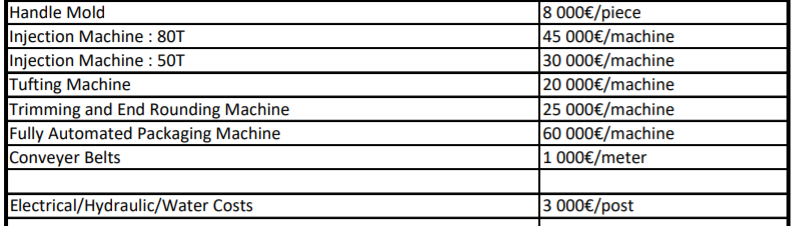
\includegraphics[scale=0.9]{Img/averageMachineCost.png}
	\caption{Average machine costs}

\end{figure}

We have 5 machines in our assembly line. We decided, for the electrical/hydraulic/water costs, that there will be a maximum of 3 machines by post, so 2 posts for one assembly line, which will cost 6 000 euros.

\begin{figure}[h]

	\centering
	\includegraphics[scale=0.6]{Img/machineCost.png}
	\caption{Machines costs for one assembly line}

\end{figure}

So, the total machine cost for one assembly line is \textbf{188 000 euros}.

We reach a total estimation cost of \textbf{272 626.96 euros} with both the human cost and the machine cost.
